\documentclass[a4paper,11pt]{article}

\usepackage{amsmath}
\usepackage{amssymb}
%\usepackage{amsthm}
\usepackage{graphicx}
\usepackage{epstopdf}
\epstopdfsetup{update}
%\usepackage{caption}
%\usepackage{subcaption}

\newcommand{\ba}{\begin{array}}
\newcommand{\ea}{\end{array}}

\newcommand{\bea}{\begin{eqnarray}}
\newcommand{\eea}{\end{eqnarray}}

\newcommand{\bc}{\begin{center}}
\newcommand{\ec}{\end{center}}

\newcommand{\ds}{\displaystyle}

\newcommand{\bt}{\begin{tabular}}
\newcommand{\et}{\end{tabular}}

\newcommand{\bi}{\begin{itemize}}
\newcommand{\ei}{\end{itemize}}

\newcommand{\bd}{\begin{description}}
\newcommand{\ed}{\end{description}}

\newcommand{\bp}{\begin{pmatrix}}
\newcommand{\ep}{\end{pmatrix}}

\newcommand{\pd}{\partial}
\newcommand{\sech}{\mbox{sech}}

\newcommand{\cf}{{\it cf.}~}

\newcommand{\ltwo}{L_{2}(\mathbb{R}^{2})}
\newcommand{\smooth}{C^{\infty}_{0}(\mathbb{R}^{2})}

\newcommand{\br}{{\bf r}}
\newcommand{\bk}{{\bf k}}
\newcommand{\bv}{{\bf v}}

\newcommand{\gnorm}[1]{\left|\left| #1\right|\right|}
\newcommand{\ipro}[2]{\left<#1,#2 \right>}

\author{Christopher W. Curtis \\
Ricardo Carretero\\
Matteo Polimeno}
\date{}
\title{Characterizing Coherent Structures in Bose-Einstein Condensates through Dynamic-Mode Decomposition}
\begin{document}
\maketitle
\section*{Introduction}
With the recent experimental observation of turbulent cascades in a Bose-Einstein Condensate (BEC) \cite{navon}, it is important to continue to better understand and characterize in as quantitative a means as possible the complex dynamics associated with turbulence in dispersive, nonlinear-wave systems.  While small-amplitude states whose statistics remain nearly Gaussian permit a relatively complete analytic characterization of turbulent cascades, embodied in the weak-wave turbulence (WWT) theory initiated in \cite{zakharov} and collected in \cite{nazarenko}, as noted in \cite{newell,cai}, the assumptions which one makes to derive results in WWT necessarily must generically break down over long-enough timescales.  

This breakdown is best characterized by the formation of long-wavelength, larger-amplitude coherent structures (CSs).  In classic, one-dimensional systems, characterizing such structures in terms of solitons is relatively straightforward; see \cite{cai}.  However, in two-dimensions, and for systems like the defocusing nonlinear Schr\"{o}dinger equation (NLSE), describing coherent structures in quantitative terms is far more challenging.  In the context of BECs, a variety of heuristic metrics to characterize CSs appeared in \cite{nazarenko2}.  In the broader context of WWT, along with classic approaches built around studying qualitative features in Fourier transforms, methods based on tracking spikes in Gaussian curvature of the solution have appeared in \cite{mordant}.  

However, as noted in \cite{nazarenko2}, CSs are difficult to visulalize in terms of physically measurable variables in BECs.  This is due in part to the role that vortices play in BECs, whereby the formation of CSs corresponds to the elimination of vortices.  This in some sense removes the most readily identifiable features of the flow, making characterization of the transition away from the WWT state difficult.  In this paper, instead, we study the use of Dynamic-Mode Decompositions (DMDs), \cite{schmid,williams,kutz}, which is a modal decomposition generated by discrete snap-shots of the temporal evolution of the BEC.  The advantage of DMDs is in their great flexibility due to their essentially being a model-free means of analyzing flows.  

As we show, by selecting the most temporally dominant modes from the DMD, we are readily able to characterize coherent states that otherwise remain undetectable in the BEC flow.  

\section*{Modelling and Weak-Wave Turbulence}

In non-dimensional coordinates (see the Appendix for details on the non-dimensionalization), we model the BEC through the use of a stochastically forced Gross--Pitaevskii (GP), or NLS, equation 
\[
i\psi_{t} = -\Delta \psi +  \left| \psi\right|^{2}\psi + \gamma_{f}({\bf x},t) - i(\nu_{h}\Delta^{2n}+\nu_{l}\tilde{\Delta}^{-2n})\psi, ~ \psi({\bf x},0)=0.
\]
Note, we always remain in the defocusing, or `dark', case.  We solve this equation with periodic boundary conditions, where the common period $2L \gg 1$ so that we have the equivalent Fourier representation of $\psi$,
\[
\psi({\bf x},t) = \sum_{{\bf k}_{mn}} a({\bf k}_{mn},t) e^{\pi i {\bf k}_{mn}\cdot {\bf x}/L}.
\]

The forcing $\gamma_{f}$ is chosen so as to be a spectrally-band limited function 
\[
\gamma_{f}({\bf x},t) = \gamma_{0}e^{2\pi i\varphi(t)}\sum_{k_{l}\leq |{\bf k}_{mn}| \leq k_{h}} e^{\pi i {\bf k}_{mn}\cdot {\bf x}/L}, ~ {\bf k}_{mn} = (m,n), 
\]
and the phase $\varphi(t)$ is such that $\varphi(t)  \sim U(0,1)$ where $U(0,1)$ denotes random variables uniformly distributed between $0$ and $1$.  Thus, our forcing is characterized by an injection range of wavenumbers via the choices of $k_{l}$ and $k_{h}$.  We likewise see that the forcing is unbiased in any particular spatial direction, so that by starting with zero-initial conditions, we see that the solution $\psi({\bf x},t)$ will largely mimick the forcing until it has reached a large enough amplitude that nonlinearity, through four-wave mixing, is able to transfer energy across Fourier modes.  This is ultimately balanced against the strength of the hyperviscosity characterized by the magnitude of $\nu_{h}$ and the hypoviscosity characterized by the magnitude of $\nu_{l}$.  

We note that the question of what a `large' domain is is somewhat ambiguous in this problem due to the forcing.  Traditionally when modelling a BEC, a length scale is set via the `healing-length' \cite{pethick}, which ultimately determines the width of vortices in the GPE.  However, to do this one must have a fixed particle number $N= \int \left|\psi\right|^{2}d{\bf x}$, but due to the forcing we necessarily have that 
\begin{align*}
\frac{1}{2}\frac{dN}{dt} = &  \mbox{Im}\left\{\int \gamma_{f}({\bf x},t) \psi^{\ast} d{\bf x} \right\}\\
& - \int \psi^{\ast}\left(\nu_{h}\Delta^{2n}+\nu_{l}\tilde{\Delta}^{-2n}\right)\psi d{\bf x}
\end{align*}
so that the particle number, and thus length scale, can change with time.  Ultimately though, a quasi-equilibrium is achieved through the balance of injection due to the forcing $\gamma_{f}$ and the particle removal/energy dissipation due to the hyper/hypoviscosity.  

By forcing the system starting from a zero-amplitude state, we hope to ultimately generate a weak-wave turbulence (WWT) state.  This is characterized as a nontrivial energy flux in wavenumber.  The associated isotropic energy density $E_{d}(k,t)$ is given by 
\[
E_{d}(k,t) = 2\pi k\omega(k)n(k,t), 
\]
where $\omega(k)$ is the dispersion relationship of the GPE, and $n(k)$ is given by 
\[
n(k,t) = \left< \left|a(\bk_{nm},t)\right|^{2}\right>, ~ \left|\bk_{nm}\right| = k.
\]
The brackets denote averaging, which in our case, assuming ergodicity, will correspond to temporally averaging the power spectra of the solution of the GPE.  

Associated with the energy density is an affiliated energy flux $\epsilon$ so that 
\[
\pd_{t} E_{d} + \pd_{k}\epsilon \sim 0.
\]
It is one of the major achievements in the WWT theory that one can derive Boltzman like kinetic equations describing the evolution of $n(k,t)$ \cite{nazarenko}.  Thus, if we characterize the WWT state as one at which the energy density is in quasi-equilibrium so that $\pd_{t}E_{d}\sim 0$, which therefore implies that $\pd_{t}n(k,t)\sim 0$, we can then distinguish equilibrium profiles of $n(k,t)$ by whether $\epsilon \sim 0$ or $\epsilon \sim c$, where c is some constant.  The zero case corresponds to no energy flux, thereby describing a thermodynamically steady state associated with the equipartion of energy.  It is the non-zero energy flux states which distinguish WWT states, and those that we are most interested in studying.  

\section*{Dynamic-Mode Decomposition}
We briefly review the details of the DMD for completeness and to better explain later results.  In DMD, we assume that any time series of a dynamical quantity of interest, denoted by $\left\{\phi_{n}\right\}_{n=1}^{\infty}$, can be described through a linear process mediated via an operator, say $A$ so that 
\[
\phi_{n+1} = A \phi_{n}.  
\] 
We treat $A$ as essentially unknowable in any direct sense, but by using the affiliated matrices $V_{1}^{N}$, where
\[
V^{N}_{1} = \left\{\phi_{1} \cdots \phi_{N} \right\}
\]
and $V_{2}^{N} = AV_{1}^{N}$, and using a Singular Value Decomposition (SVD) on $V_{1}^{N}$ so that $V_{1}^{N} = U\Sigma W^{\dagger}$, we see that 
\[
U^{\dagger}AU = \tilde{S}, ~ \tilde{S} = U^{\dagger}V_{2}^{N}W\Sigma^{-1}.
\]
Thus by computing the associated eigenvalues and eigenvectors of $\tilde{S}$, say $\mu_{j}$ and $\tilde{\phi}_{j}$respectively, then for $N$ large enough with sufficiently controlled spacing in the time-series, these eigenvalues and eigenvectors will approximate those of $A$.  Likewise, this allows us to write the approximation 
\[
\phi_{n} = \sum_{j=1}^{N} b_{j}\mu_{j}^{n \delta t} U\tilde{\phi}_{j}
\]
where $\delta t$ represents the time spacing between elements of the time series.  Thus, by examining the terms $\left|\tilde{b}_{N}\right|$ where
\[
\tilde{b}_{N} = b_{j} \mu_{j}^{N \delta t},
\]
we can effectively rank the relative importance of the dynamic modes represented by $\tilde{\phi}_{j}$, thereby providing a method of reducing complicate data to a far smaller subspace of phenomena.  

\subsection*{Validation}
To better understand the results of using DMD and what the impacts are for various selection strategies, we study a relatively simple flow.  Removing the forcing and hypo/hyperviscosity, we use as initial condition to the GPE
\[
\psi({\bf x},0) = \prod_{j=1}^{N_{v}}\prod_{k=1}^{N_{v}} \phi(r_{jk})e^{is_{jk}\theta_{jk}}, 
\]
where
\[
s_{jk} = (-1)^{j+k}, ~ r_{jk} = \left|{\bf x} - (x_{j},y_{k}) \right|, ~ \theta_{jk} = \tan^{-1}\left(\frac{y-y_{k}}{x-x_{j}} \right),
\]
and $\phi(r)$ solves the circularly symmetric NLS equation
\[
\pd_{r}^{2}\phi  + \frac{1}{r}\pd_{r}\phi - \frac{1}{r^{2}}\phi + \phi(1-\phi^{2}) = 0, ~ \lim_{r\rightarrow\infty} \phi(r) = 1.
\]
Thus, the initial condition consists of a product of unit strength vortices of alternating orientations.  By setting the vortex centers $(x_{j},y_{k})$ to be 
\[
x_{j} = \frac{1}{2} - 4N_{v} + 8j, ~ y_{k} = \frac{1}{2}-4N_{v} + 8k 
\]
then we begin with an equispaced array of vortices with the vortices well seperated in distance so as to allow them to remain readily observable over reasonable lengths of simulation time.  

Choosing the alternating pattern of vortex orientations allows us to use periodic boundary conditions, and thus standard Fourier based pseudo-spectral schemes to study this problem numerically.  We then choose, so as to be consistent with the later simulations in this paper, $L=128$ and the number of modes to be $K_{T}=512$, giving a spatial step of $\delta x = 256/512=1/2$.  Using a two-stage Runge Kutta (RK) scheme with time step $\delta\tilde{t} = .05$, we then evolve the above initial condition forward $t_{f}=20$ units of time.  Choosing $N_{v}=2$ so that we start with an array of four vortices then generates the amplitude plot seen in Figure \ref{fig:frvtx} (a).
\begin{figure}
\centering
\begin{tabular}{cc}
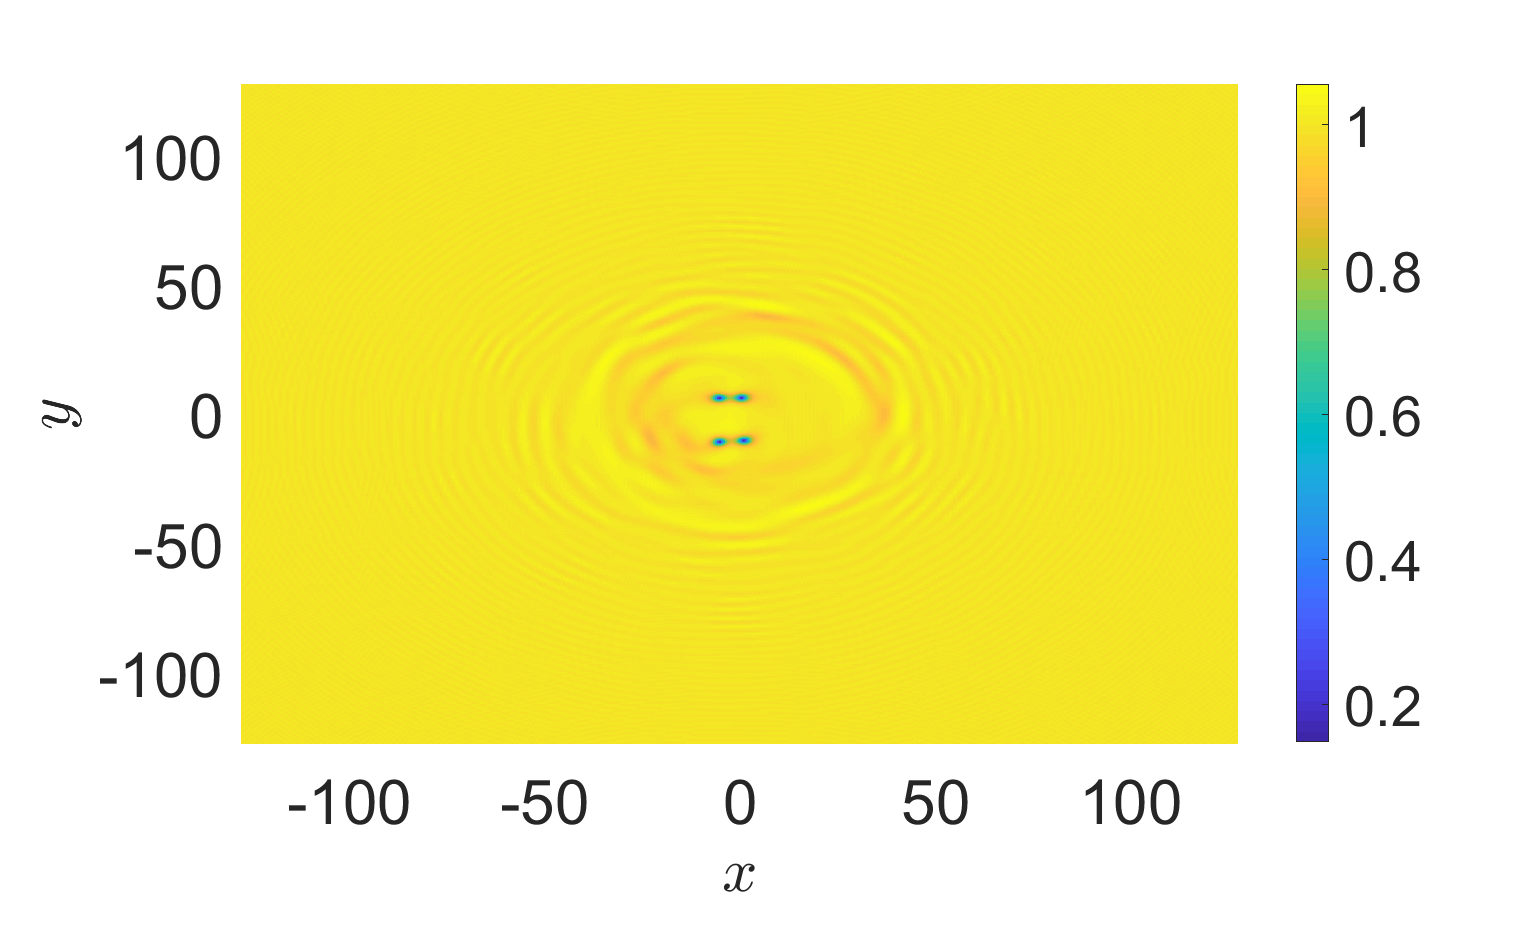
\includegraphics[width=.52\textwidth]{four_vortex_tf_20_K_256_Llx_128} &\hspace{-24pt} 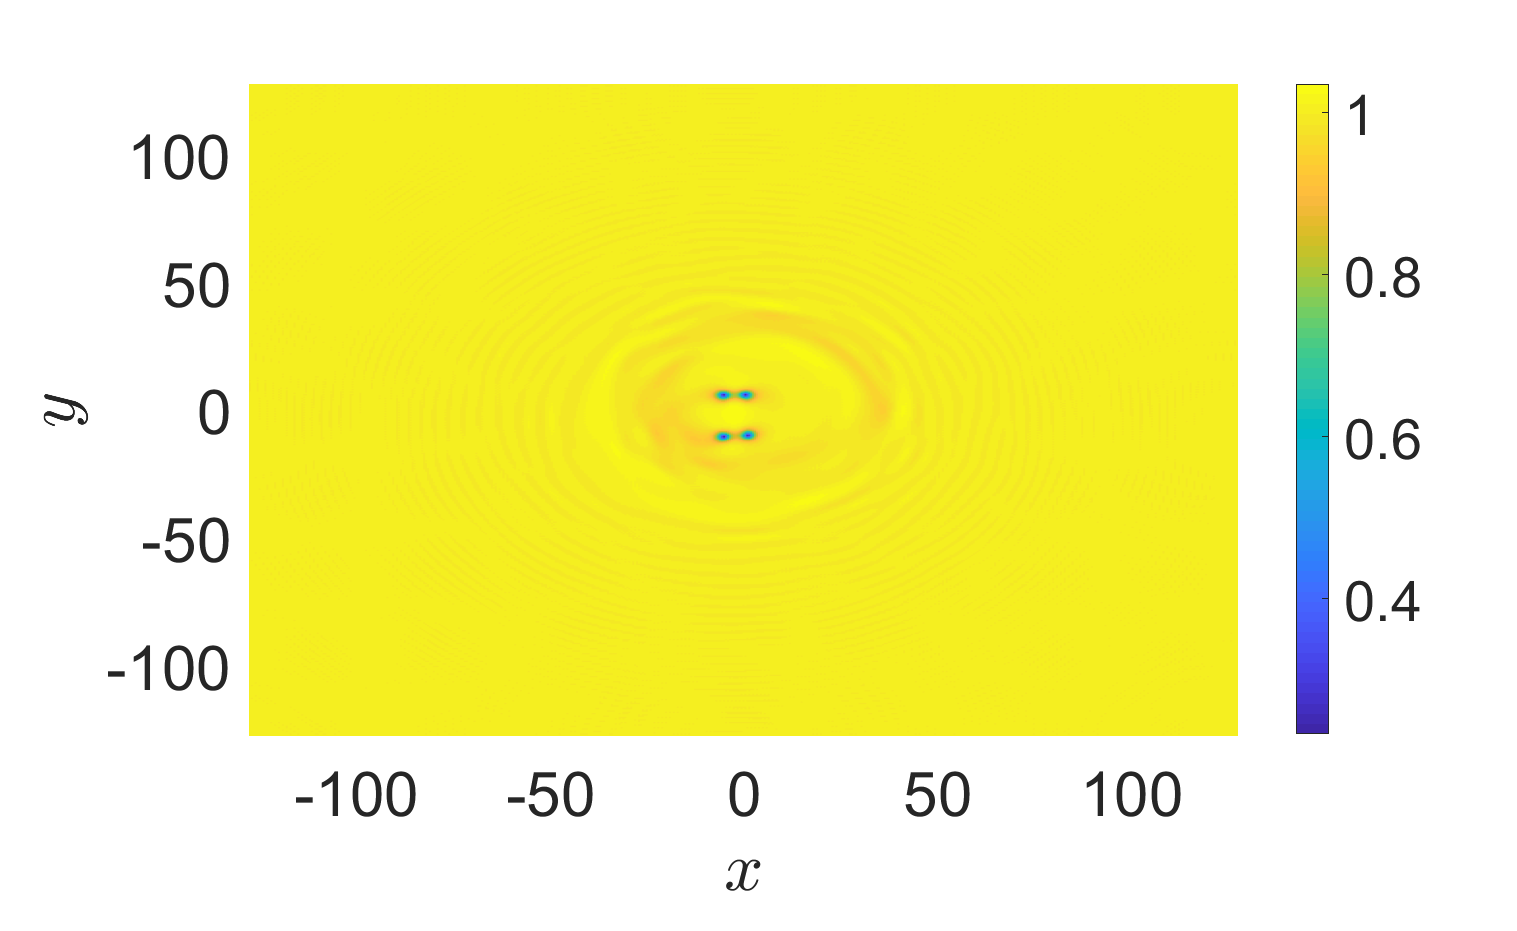
\includegraphics[width=.52\textwidth]{dmd1_four_vortex_tf_20_K_256_Llx_128}\\
(a) & (b)\\
 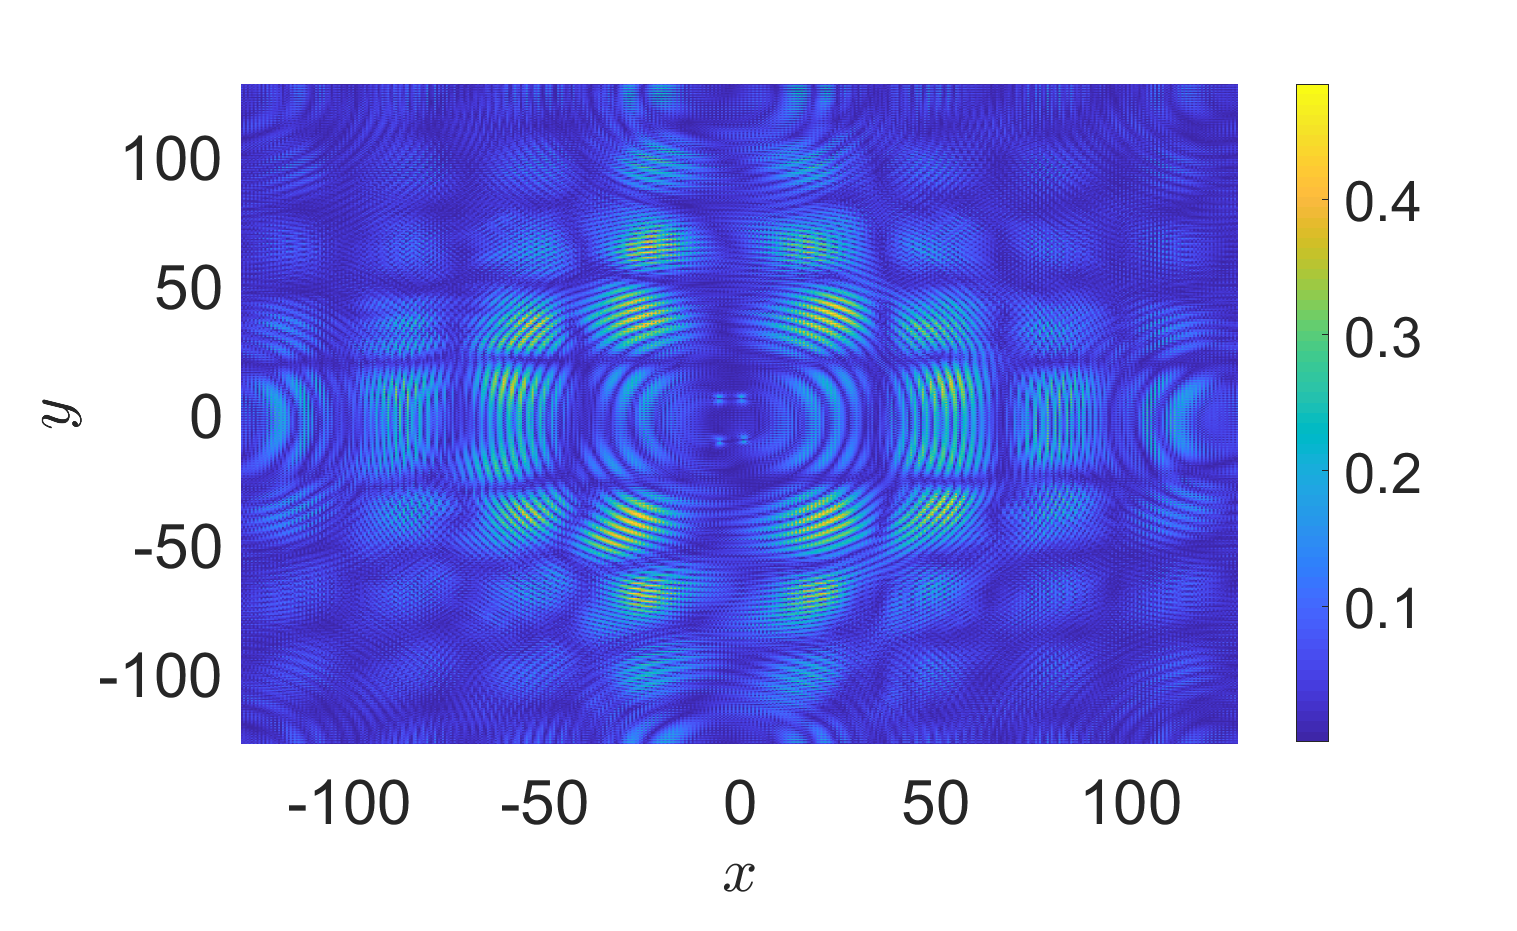
\includegraphics[width=.52\textwidth]{dmd2_four_vortex_tf_20_K_256_Llx_128} &\hspace{-24pt} 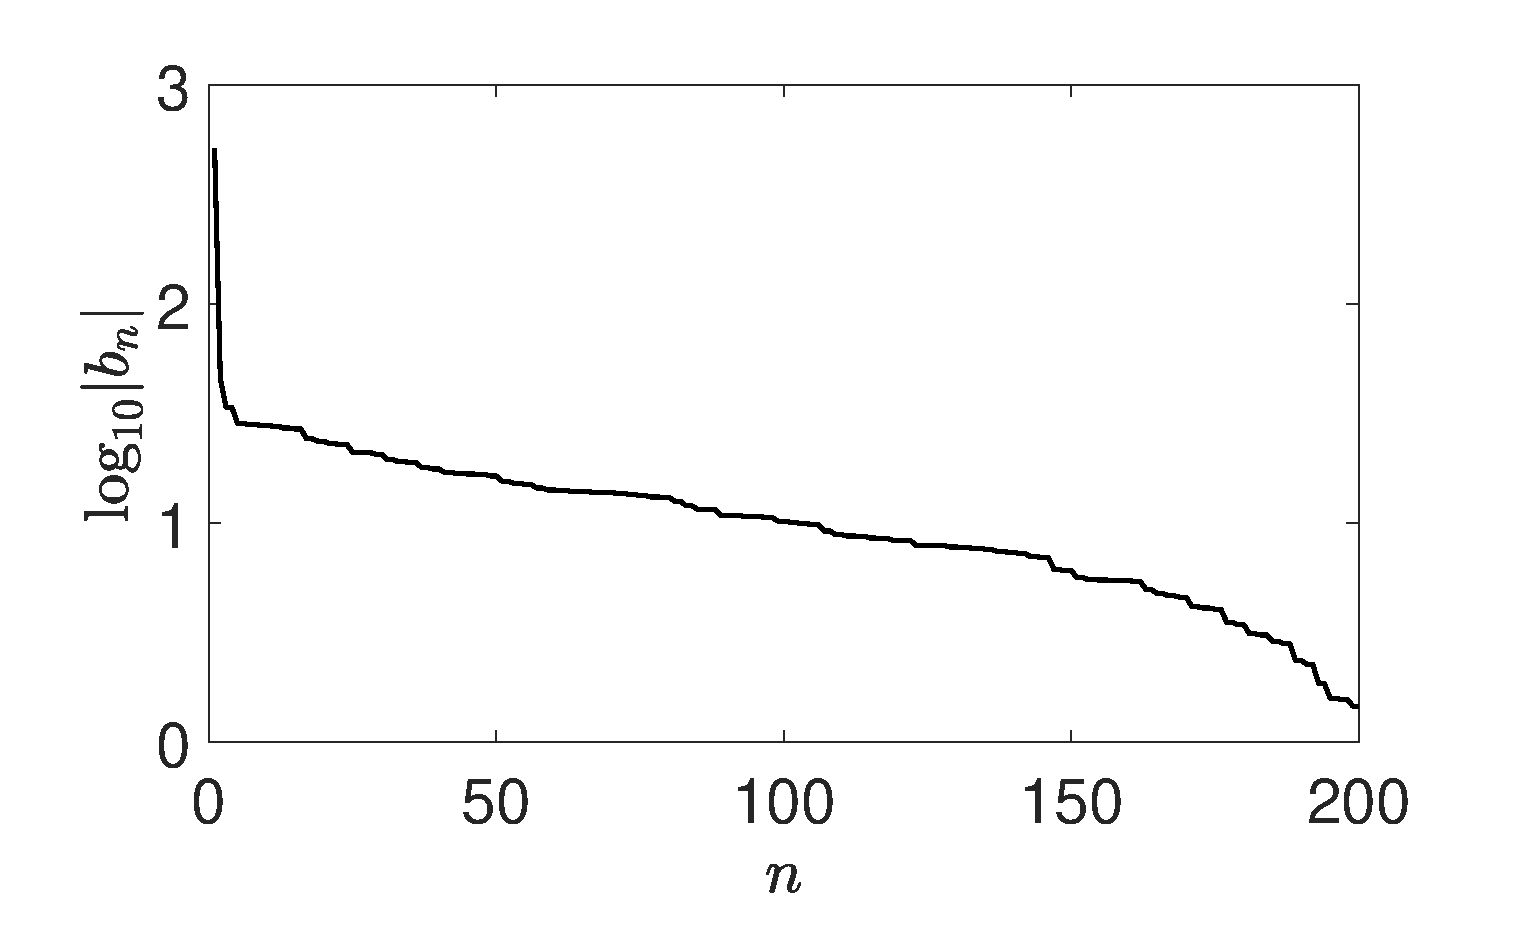
\includegraphics[width=.52\textwidth]{dmd_mags_tf_20_K_256_Llx_128}\\
(c) & (d) 
\end{tabular}
\caption{The amplitude $\left|\psi(x,y,t_{f})\right|$ (a), and magnitudes of the first two most dominant DMD modes, (b) and (c) for an initial array of four vortices.  }
\label{fig:frvtx}
\end{figure}

As can be seen, on the relatively short time scales examined here, the vortices hardly move, though they do induce a significant amount of sound waves due to their mutual interactions.  If we then perform a DMD on the amplitude $\left|\psi({\bf x},t)\right|$ for $t\geq t_{f}/2$, where the sampling is done every five simulation time steps, we find that the magnitudes $\tilde{b}_{N}$ are readily segregated so that one mode is markedly more dominant than any other.  This mode is shown in Figure \ref{fig:frvtx} (b), which as can be seen, is mostly identical to the true amplitude $\left|\psi({\bf x},t_{f})\right|$ shown in Figure \ref{fig:frvtx} (a).  This intuitively makes sense given the relatively slowly evolution seen, thereby making the most significant DMD mode an effective fixed point of the unknown mapping $A$.  Our choice for the mode plotted in Figure \ref{fig:frvtx} (b) is made by comparing the relative magnitudes of the modes $\tilde{b}_{N}$ shown in Figure \ref{fig:frvtx} (d).  As seen, there is clearly one mode that is an order of magnitude stronger than the rest, and this relative importance is reflected in the nearly identical plots seen in Figures \ref{fig:frvtx} (a) and (b).

So, in many respects, this shows how powerful the DMD approach can be.  In contrast though, we see that moving to the next most significant mode, shown in Figure \ref{fig:frvtx} (c), does not readily enhance our understanding of the details of the flow not captured by the most significant mode.  Further, we see in Figure \ref{fig:frvtx} (d) that there is a long tail consisting of over a hundred modes all of relatively equal importance.  Thus, while one mode readily captures the most salient features of the flow, to get finer resolution would require large numbers of modes thereafter.  Thus, moving forward, we see that it is important to seperate the magnitudes of $\tilde{b}_{N}$ into various groupings of similar magnitudes.  
 
\section*{Characterizing Coherent States}

\subsection*{Down-Scale Weak Turbulence Cascades}
In this case, we take $k_{l}=4$, $k_{h}=6$, and $\gamma_{0}=2.1\times 10^{-3}$.  To recreate the WWT results of \cite{nazarenko2}, we keep both hypo and hyperviscosity in place.  The results of this are seen in Figure \ref{fig:ampcomplfwwt}.    Here, and using Figure \ref{fig:ampcomplfwwt} (d) for guidance, we see that a single DMD mode carries the vast majority of the field, with the second most prominent mode far smaller in magnitude than the first.  While a degree of regularity is seen in the first DMD mode, there is no readily recognizable large scale structure, which is consistent with the dynamics being in the WWT regime with the specific formation of long-wavelength CSs being prohibited through the action of the hyopviscosity.
\begin{figure}
\centering
\begin{tabular}{cc}
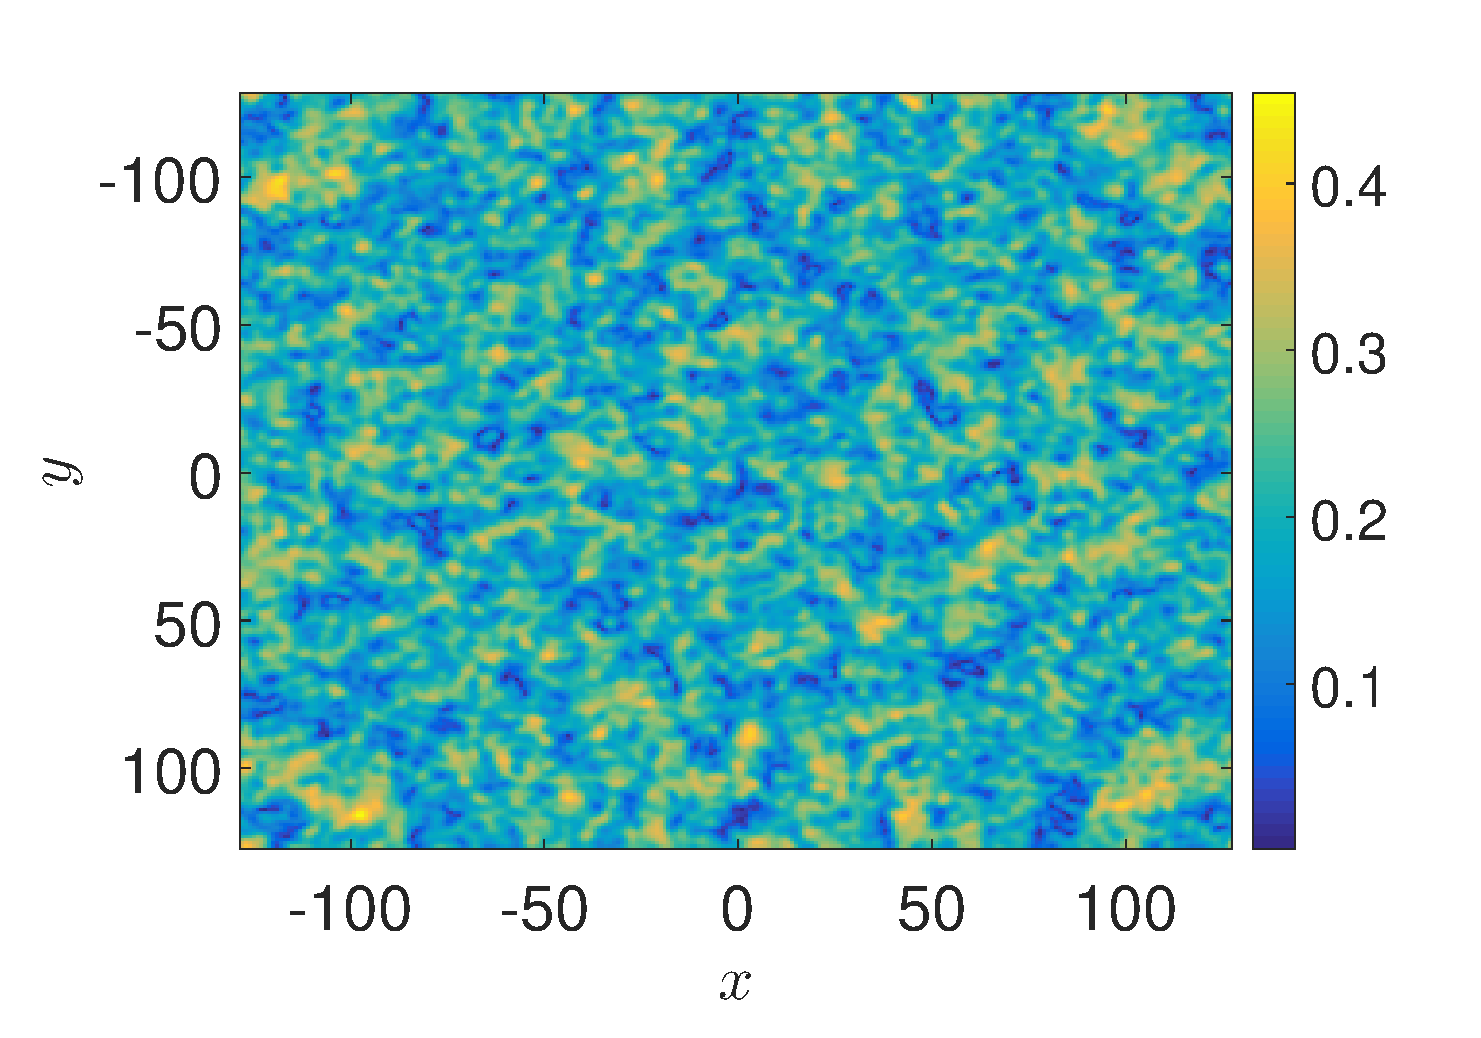
\includegraphics[width=.52\textwidth]{amplitude_wwt_K_128_Lx_128_tf_1pt5e4} &\hspace{-24pt} 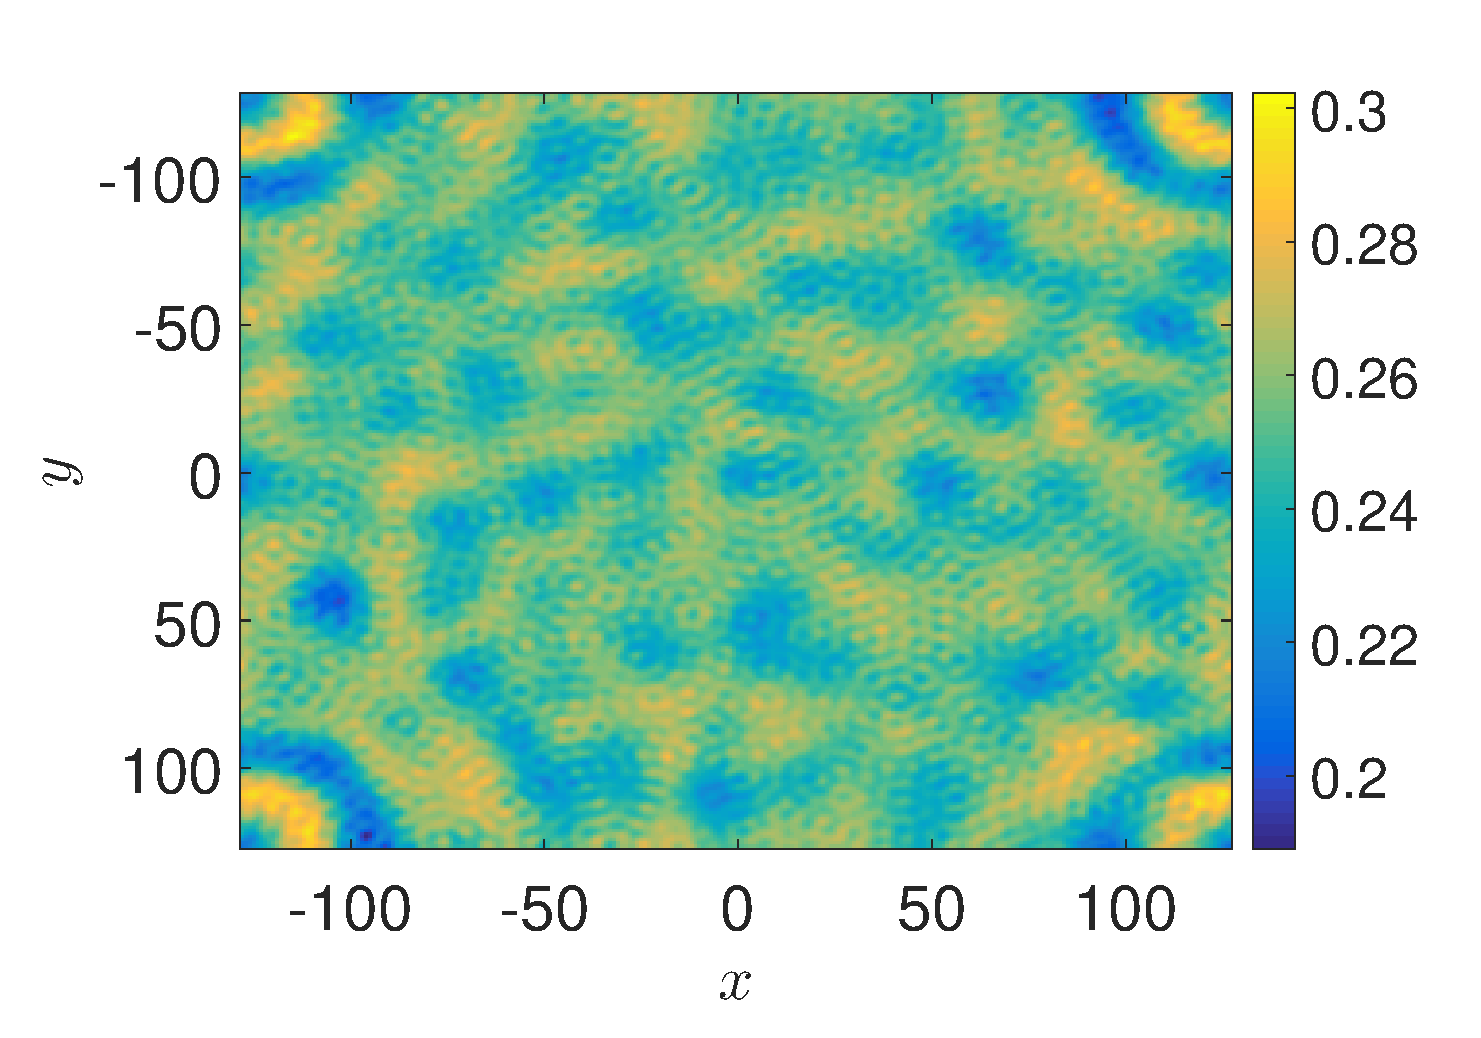
\includegraphics[width=.52\textwidth]{dmd1_amplitude_wwt_K_128_Lx_128_tf_1pt5e4} \\
(a) & (b)\\
\includegraphics[width=.52\textwidth]{dmd2_amplitude_wwt_K_128_Lx_128_tf_1pt5e4} &\hspace{-24pt} \includegraphics[width=.52\textwidth]{dmd_mags_wwt_K_128_Lx_128_tf_1pt5e4}\\
(c) & (d) 
\end{tabular}
\caption{The amplitude $\left|\psi(x,y,t_{f})\right|$ (a), and magnitudes of the first two most dominant DMD modes, (b) and (c) and plot of $\left|\tilde{b}_{N}\right|$ for $k_{l}=4$, $k_{h}=6$, $\gamma_{0}=2.1\times 10^{-3}$.  }
\label{fig:ampcomplfwwt}
\end{figure}

If we remove the hypoviscosity, thereby allowing for saturation in longer-wavelengths to occur, we see in Figure \ref{fig:ampcomplf} that coherent structures form, and are readily identifiable via examing the first two modes of the DMD.  We see in Figure \ref{fig:ampcomplf} (d) that the first two modes carry the large majority of the weight in the DMD, thereby providing a ready lower dimensional representation of the dynamics.  
\begin{figure}
\centering
\begin{tabular}{cc}
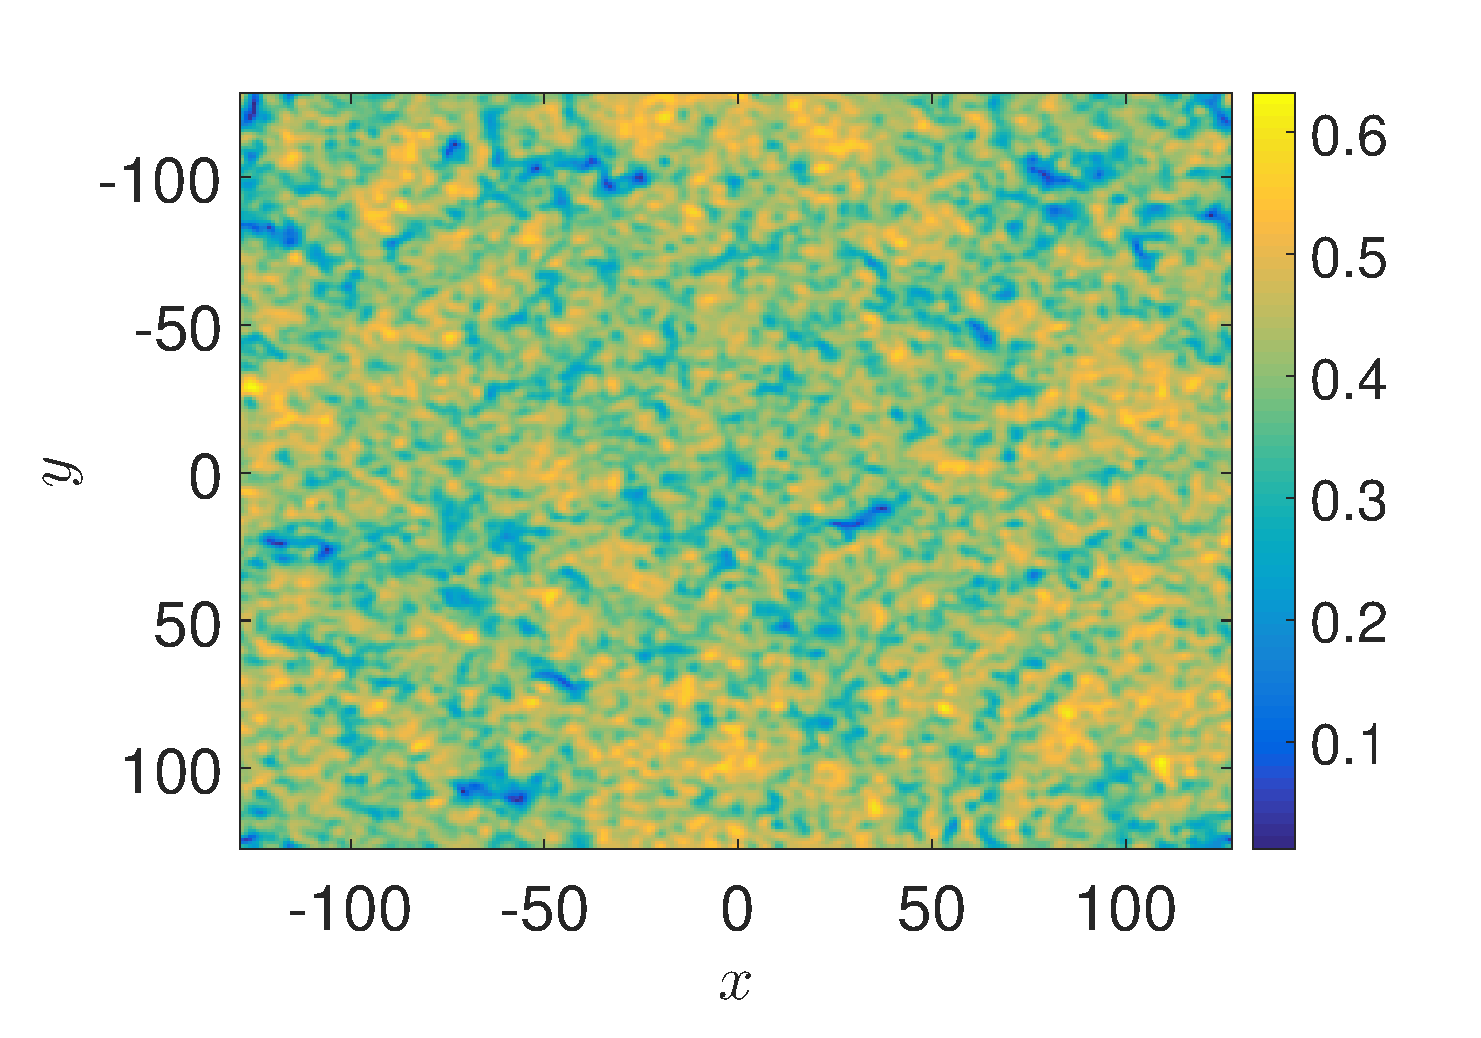
\includegraphics[width=.52\textwidth]{amplitude_K_128_Lx_128_tf_1pt5e4} &\hspace{-24pt} \includegraphics[width=.52\textwidth]{dmd1_amplitude_K_128_Lx_128_tf_1pt5e4}\\
(a) & (b)\\
\includegraphics[width=.52\textwidth]{dmd2_amplitude_K_128_Lx_128_tf_1pt5e4} &\hspace{-24pt} 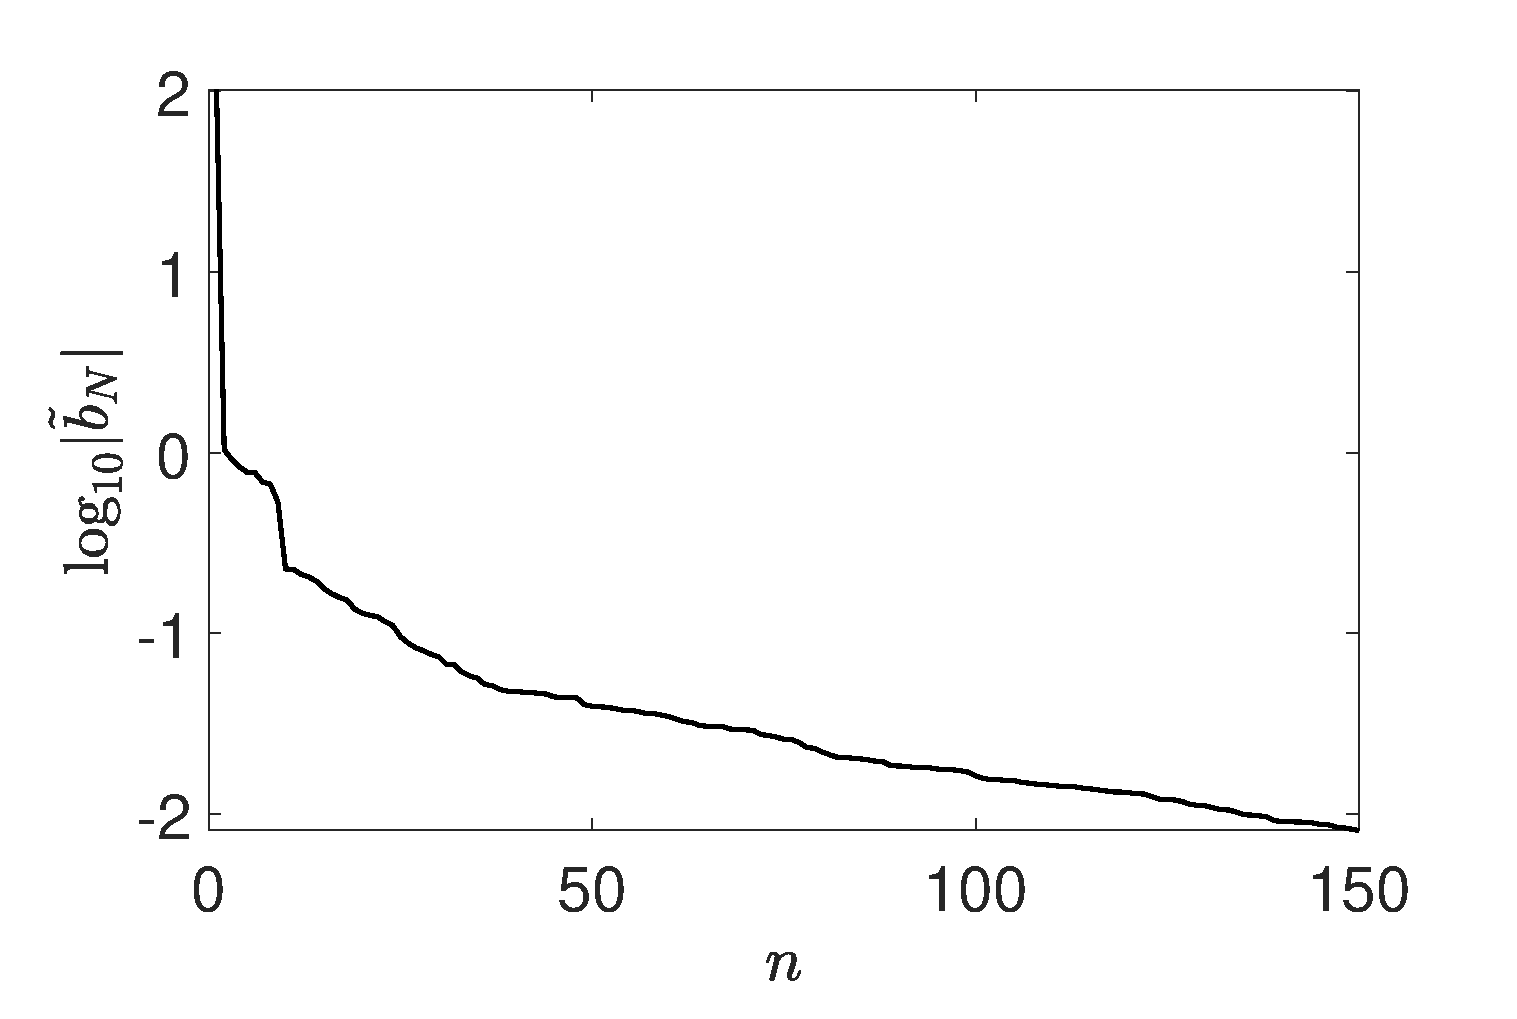
\includegraphics[width=.52\textwidth]{dmd_mags_K_128_Lx_128_tf_1pt5e4}\\
(c) & (d)
\end{tabular}
\caption{The amplitude $\left|\psi(x,y,t_{f})\right|$ (a), and magnitudes of the first two most dominant DMD modes, (b) and (c), and plot of $\left|\tilde{b}_{N}\right|$ (d) for $k_{l}=4$, $k_{h}=6$, $\gamma_{0}=2.1\times 10^{-3}$. Note the relative increase in the magnitude of the second most significant DMD mode.}
\label{fig:ampcomplf}
\end{figure}

\subsection*{Long-Wavelength Saturation and Coherent States}
In this case, we let $k_{l}=60$ and $k_{h}=63$, so that the injection range of the forcing is at a relatively high-frequency.  We remove the hypoviscosity, thereby allowing for the saturation of energy at long wavelengths.  Increasing the forcing amplitude to $\gamma_{0}=1.6\times 10^{-3}$, we allow the simulation to run up to $t_{f}=1.5\times 10^{4}$ units of non-dimensional time.  We perform a DMD and compare the magnitude $\left|\psi\right|$ to that of the first two most dominant dynamic modes in Figure \ref{fig:ampcomphf}
\begin{figure}
\centering
\begin{tabular}{cc}
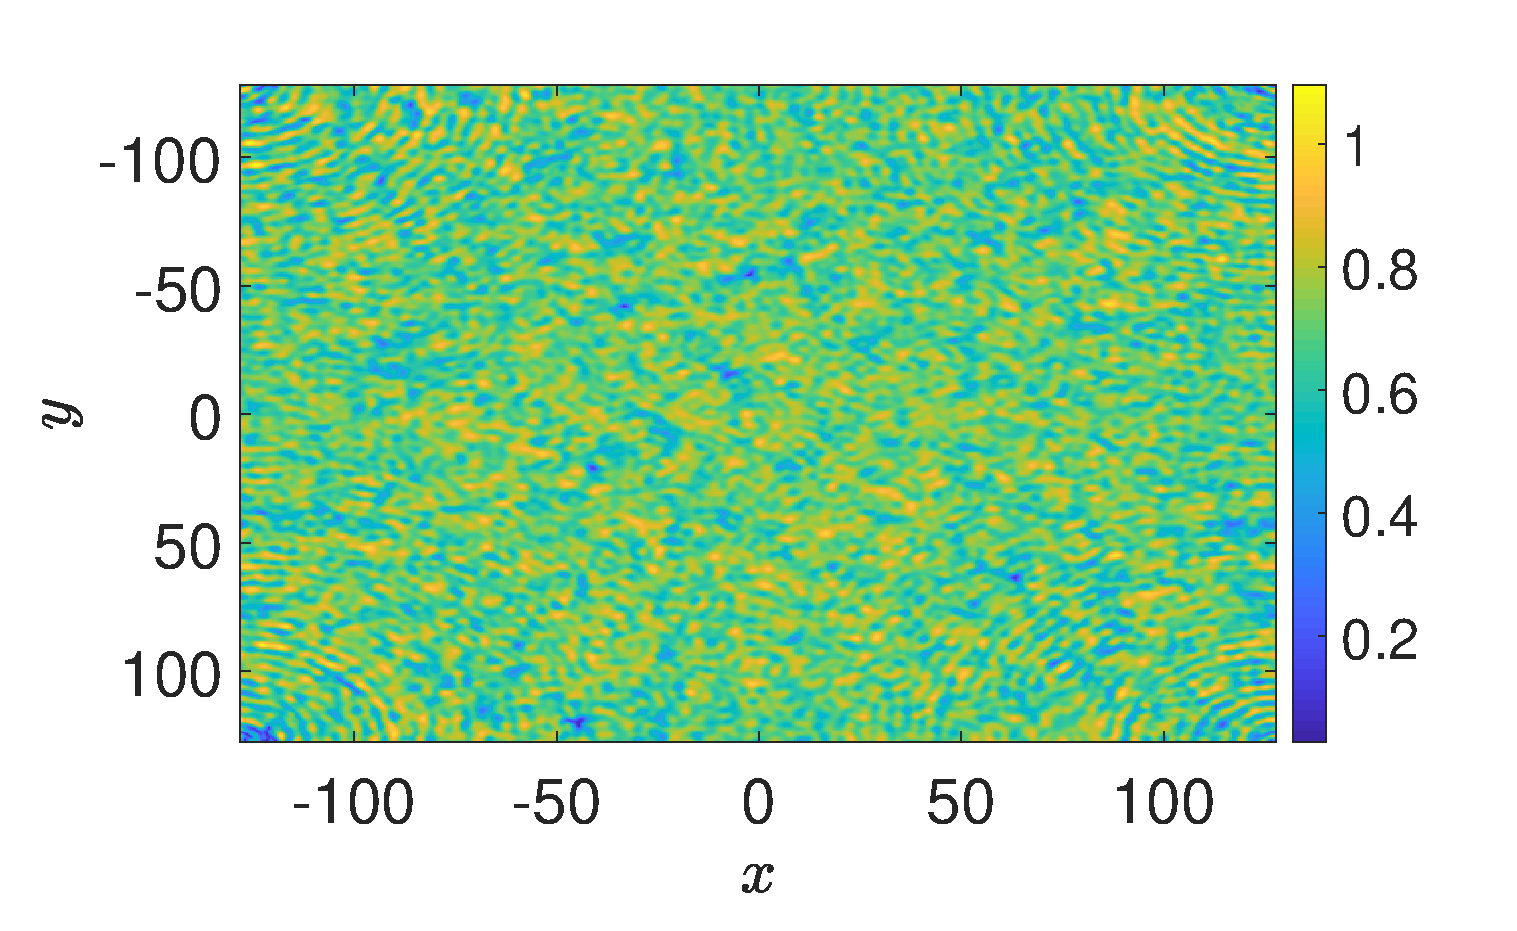
\includegraphics[width=.51\textwidth]{amplitude_hfforce_K_256_Lx_128_tf_1pt5e4} &\hspace{-20pt} 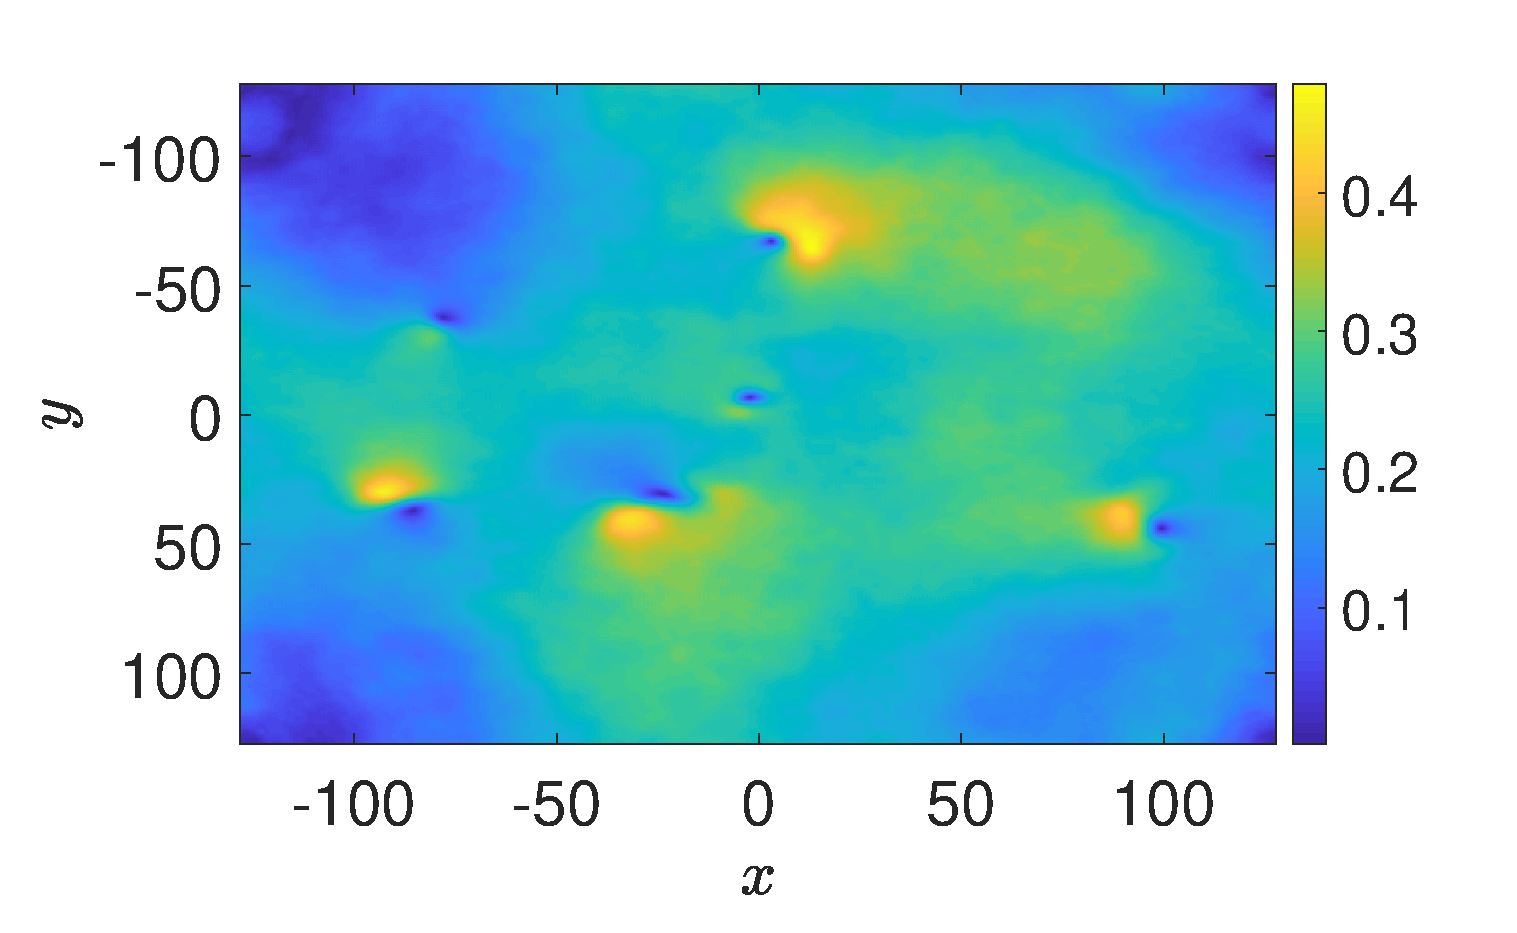
\includegraphics[width=.51\textwidth]{dmd1_amplitude_hfforce_K_256_Lx_128_tf_1pt5e4} \\
(a) & (b)\\
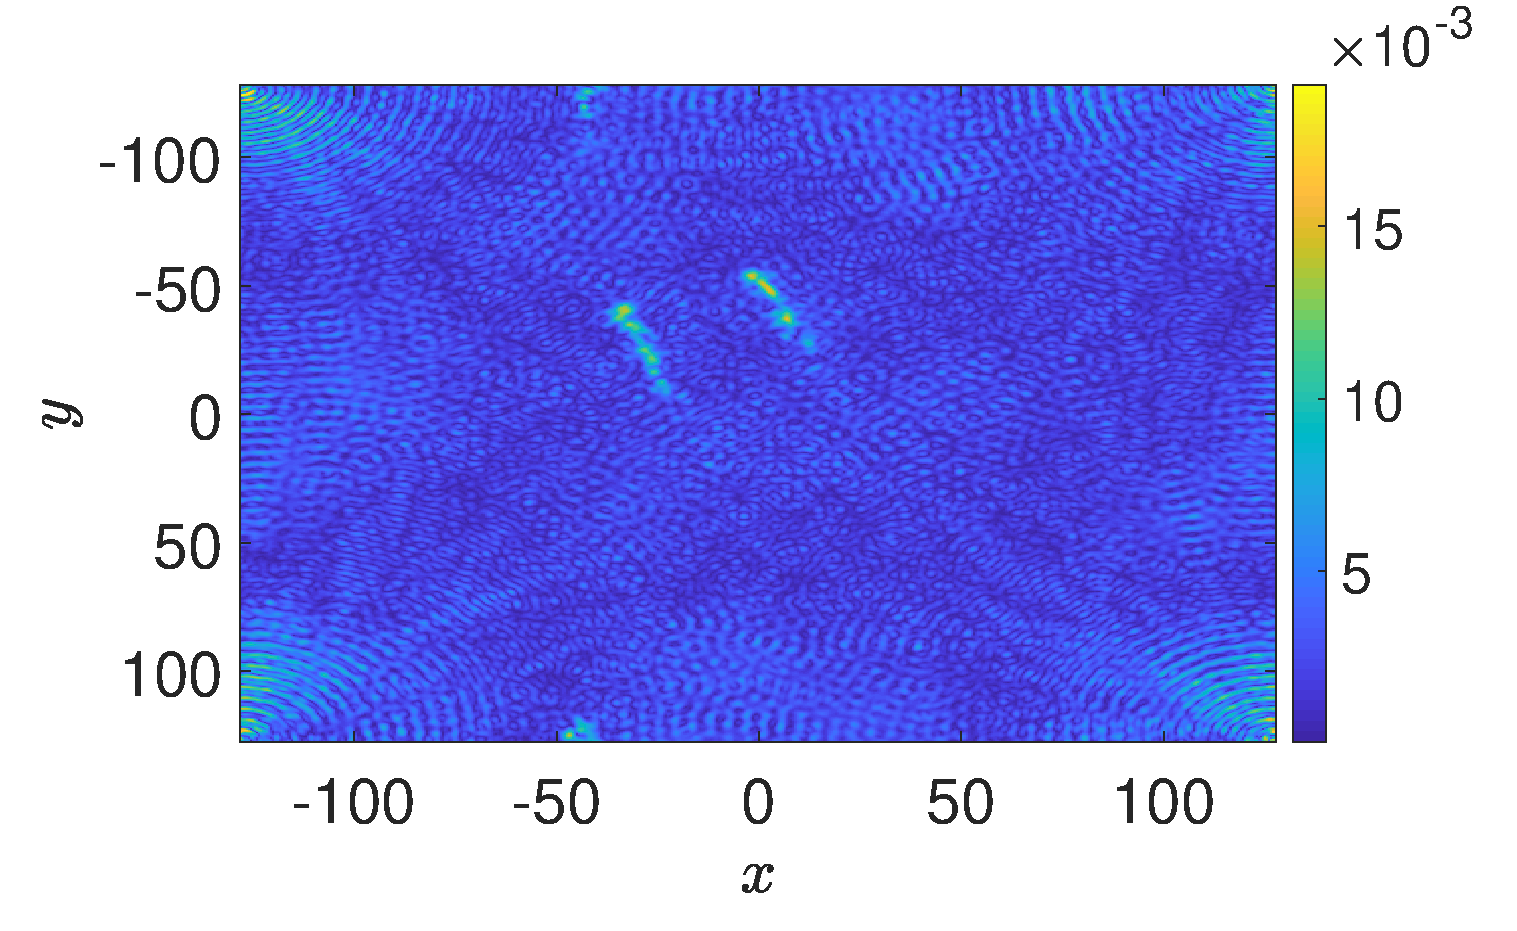
\includegraphics[width=.51\textwidth]{dmd2_amplitude_hfforce_K_256_Lx_128_tf_1pt5e4} &\hspace{-20pt} 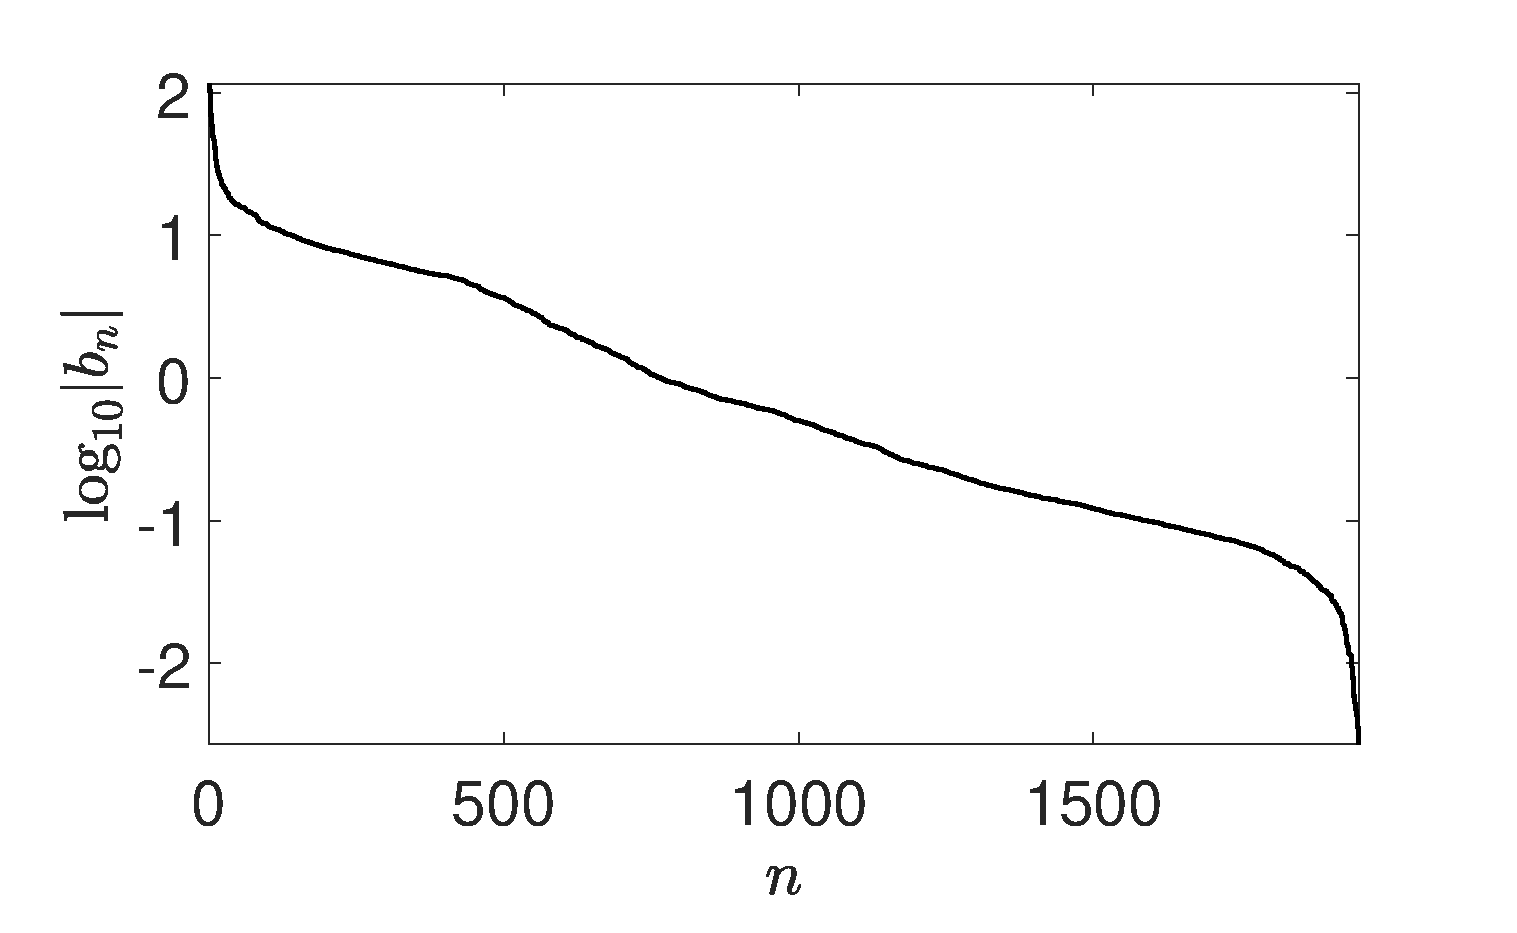
\includegraphics[width=.51\textwidth]{dmd_mags_hfforce_K_256_Lx_128_tf_1pt5e4}\\
(c) & (d)
\end{tabular}
\caption{The amplitude $\left|\psi(x,y,t_{f})\right|$ (a), and magnitudes of the  first two most dominant DMD modes, (b) and (c), and plot of $\left|\tilde{b}_{N}\right|$ (d) for $k_{l}=60$, $k_{h}=63$, $\gamma_{0}=1.6\times 10^{-3}$. }
\label{fig:ampcomphf}
\end{figure}
As can be seen, the two most dominant DMD modes clearly isolate vortices while also displaying an overall more coherent, long-wavelength driven structure which would be affiliated with the notion of a CSs put forward at the beginning of the paper.  If we likewise look at a plot of $\left|\tilde{b}_{N}\right|$ in Figure \ref{fig:ampcomphf} (d).
\section*{Conclusion}

\section*{Appendix}
With units, our model of a BEC is given by the following Gross--Pitaevksii equation (GPE)
\[
i\hbar\psi_{t} = -\frac{\hbar^{2}}{2m}\Delta \psi + g\left| \psi\right|^{2}\psi, ~ g = \frac{4\pi \hbar^{2}a_{s}}{m}
\]
where $a_{s}$ is the `scattering length', and with the clear understanding that $\left|\psi\right|^{2}dxdy$ describes probabilities in the sense that 
\[
\int |\psi|^{2}dxdy = N,
\]
where we take $N$ to be the total number of particles under consideration.  Introducing the non-dimensionalizations 
\[
\tilde{x} = x/\lambda, ~ \tilde{y} = y/\lambda, ~ \tilde{t} = t/T, 
\]
and choosing
\[
\lambda^{2} = \frac{1}{8\pi |a_{s}|}, ~ T = \frac{m}{4\pi\hbar |a_{s}|}, 
\] 
then gives us
\[
i\psi_{t} = -\Delta \psi + \sigma\left| \psi\right|^{2}\psi,  ~\sigma = \mbox{sgn}(a_{s}).
\]

\bibliography{wwt}
\bibliographystyle{unsrt}

\end{document}